\documentclass[12pt,halfline,a4paper]{ouparticle}

\begin{document}

\title{Background of Navier-Stokes Equations, Projection Method and Finite Volume Method} 

\author{%
\name{Li Ruixiang}
\email{\texttt{liruixiang@zju.edu.cn}}
}
\date{}




\maketitle
\tableofcontents
\newpage




\section{Phsical Background}
Navier-Stokes方程是流体力学中的动量守恒方程,简单的说,单位时间内控制体内动量的变化量等于流入/流出控制体的流体引起的动量变化量加上外力引起的动量变化量,我们依次考虑各个部分的动量变化,并使用以下记号:$V$表示控制体,$S$表示控制体的表面,法向量$\mathbf{n}$指向外侧.
\subsection*{控制体内动量的变化量}
考虑体积微元$\text{d} V$,其动量为$\rho \text{d} V \boldsymbol{u}$,其中$\rho$为流体密度,$\boldsymbol{u}$为流体速度,则单位时间控制体内内量的变化量为$\int_{V}\frac{\partial}{\partial t}\rho \boldsymbol{u} \text{d} V$.
\subsection*{流入/流出控制体的流体的动量变化量}
单位时间内流入/流出控制体的流体的动量变化量为$-\int_{S} \rho \boldsymbol{u} (\boldsymbol{u} \cdot \mathbf{n}) \text{d} S$,其中$\mathbf{n}$为控制体表面的法向量,负号是因为法向量向外.
\newline
利用Divergence Theorem,我们可以将面积分转化为体积分,即
\begin{equation}\label{eq:convection}
    \begin{aligned}
        (\int_{S} \rho \boldsymbol{u} (\boldsymbol{u} \cdot \mathbf{n}) \text{d} S)_d &= \int_{S} \rho u_d (\boldsymbol{u} \cdot \mathbf{n}) \text{d} S
        \\
        &=\int_{S} \rho  (u_d\boldsymbol{u} \cdot \mathbf{n}) \text{d} S\\
        &=\int_{V} \nabla \cdot (\rho u_d \boldsymbol{u}) \text{d} V\\
        &=\int_{V} (\rho u_d\nabla \cdot \boldsymbol{u}+ \rho (u\cdot\nabla)u_d )\text{d} V\\
        \int_{S} \rho \boldsymbol{u} (\boldsymbol{u} \cdot \mathbf{n}) \text{d} S &= \int_{V} \rho \boldsymbol{u} \cdot \nabla \boldsymbol{u} \text{d} V 
\end{aligned}
\end{equation}

\subsection*{外力引起的动量变化量}
外力包括重力,粘性力和压力.其中重力为体积力,粘性力和压力为表面力.我们依次考虑各个部分:
\subsubsection*{Body Force}
重力场中,单位质量流体受到的重力为$\mathbf{g}$,则控制体内流体受到的重力为$\int_V \rho \mathbf{g} \text{d} V$.
\subsubsection*{Surface Force}
\begin{figure}[h] % 'h' 表示这里插入图片
    \centering
    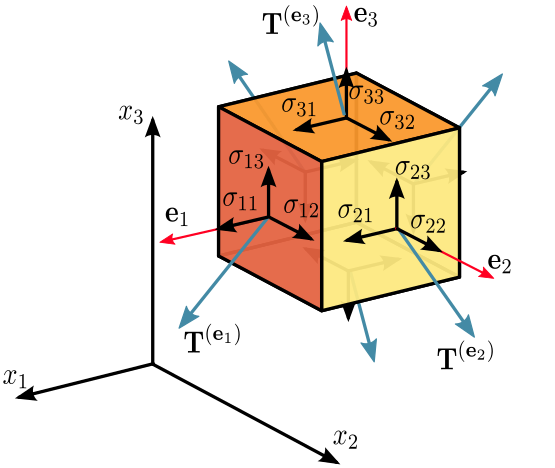
\includegraphics[width=0.5\textwidth]{figure/stress_tensor.png}
    \caption{应力张量示意图,作用在控制体的表面}  
    \label{fig:stress_tensor}  
\end{figure}
$\tau$为应力张量.
$$\tau = \begin{pmatrix}
\tau_{xx} & \tau_{xy} & \tau_{xz} \\
\tau_{yx} & \tau_{yy} & \tau_{yz} \\
\tau_{zx} & \tau_{zy} & \tau_{zz} \\
\end{pmatrix}$$
则对应的动量变化量为$\int_{S} \tau \cdot \mathbf{n} \text{d} S$.利用散度定理转化为体积分,即$\int_{S} \tau \cdot \mathbf{n} \text{d} S = \int_{V} \nabla \cdot \tau \text{d} V$.
\newline
由Stokes Hypothesis,我们有$\tau = -(p + \frac{2}{3}\nabla \cdot \boldsymbol{u} )I + \nu (\nabla \boldsymbol{u} + (\nabla \boldsymbol{u})^T)$,其中$p$为压力,$\nu$为粘性系数.
\newline
对于不可压流体满足:$\nabla \cdot \boldsymbol{u} = 0$.这是因为流入控制体内的流体等于流出控制体内的流体$\int_S \boldsymbol{u}\cdot \mathbf{n} \text{d} S = \int_V \nabla \cdot \boldsymbol{u} \text{d}V = 0$
\newline
$$\int_{V} \nabla \cdot \tau \text{d} V = \int_V (-\nabla p + \nu ( \nabla^2 \boldsymbol{u} + \nabla (\nabla \cdot \boldsymbol{u})) )\text{d} V$$
\newline
其中RHS的最后两项推导利用
% 以下记号$$\nabla = \begin{pmatrix}
% \frac{\partial}{\partial x} \\
% \frac{\partial}{\partial y} \\
% \frac{\partial}{\partial z} \\
% \end{pmatrix},\nabla \cdot = (\frac{\partial}{\partial x},\frac{\partial}{\partial y},\frac{\partial}{\partial z} ),\boldsymbol{u} = (u,v,w)$$
Einstein求和约定,$\tau_{ij} = \delta_{ij}(-p) + \nu(\frac{\partial v_i}{\partial x^j}+\frac{\partial v_j}{\partial x^i})$.
\begin{equation*}
\begin{aligned} 
    \nabla \cdot \tau  &= \frac{\partial}{\partial x^i}\tau_{ji} = \frac{\partial}{\partial x^i}\tau_{ij}  \\
    &= \frac{\partial}{\partial x^i} \delta_{ij}p + \frac{\partial}{\partial x^i}\nu(\frac{\partial u_i}{\partial x^j}+\frac{\partial u_j}{\partial x^i}) \\
    &= -\frac{\partial}{\partial x^j}p + \nu(\frac{\partial^2 u_i}{\partial x^j \partial x^i} + \frac{\partial^2 u_j}{\partial x^i \partial x^i}) \\
    &= -\nabla p + \nu(\nabla (\nabla \cdot \boldsymbol{u}) + \nabla^2 \boldsymbol{u} )
\end{aligned}
\end{equation*}
最终我们得到了不可压缩流体的Navier-Stokes方程:
\begin{equation*}
\begin{aligned}
    \rho  \frac{\partial \boldsymbol{u} }{\partial t} &= -\boldsymbol{u} \cdot \nabla \boldsymbol{u}  + \rho \mathbf{g} -\nabla p + \nu \nabla^2 \boldsymbol{u} \\
    \nabla \cdot \boldsymbol{u} &= 0
\end{aligned}
\end{equation*}
\section{Gepup}
\subsection{Projection Method}
\begin{equation}\label{eq:ns}
    \begin{aligned}
        \frac{\partial \boldsymbol{u} }{\partial t}&= -\boldsymbol{u} \cdot \nabla \boldsymbol{u}  + \mathbf{g} -\nabla p + \nu \nabla^2 \boldsymbol{u},\; \text{in}\; \Omega \times (0,+\infty)\\
        \nabla \cdot \boldsymbol{u} &= 0, \text{in} \;\Omega \times (0,+\infty)
    \end{aligned}
    \end{equation}
现在考虑在空间区域$\Omega \subset \mathbb{R}^D$内的Navier-Stokes方程\eqref{eq:ns}中,由于不可压条件是个限制条件,我们使用投影法将速度分解为无源场和一个梯度场,从而避免这个限制条件.
\subsubsection{Helmholtz Decomposition Theorem}
Helmholtz Decomposition Theorem告诉我们,有界区域$\Omega\subset\mathbb{R}$上的任意充分光滑向量场$v^*$可以唯一地分解为无源场和无旋场的和,即$v^* = v + \nabla \phi$,其中$\nabla \cdot v = 0$,而$\phi$为标量场.可以通过求解Poisson方程得到
\begin{equation}
    \begin{aligned}
        \Delta \phi &= \nabla \cdot v^* \quad \text{in} \; \Omega\\
        n \cdot \nabla \phi &= \nabla \cdot (v^*-v) \quad \text{on} \; \partial \Omega
    \end{aligned}
\end{equation}
\subsubsection{Leray-Helmholtz Projection Operator}
我们定义Leray-Helmholtz Projection Operator为
\begin{equation}\label{eq:Leray_Projection}
    \mathscr{P}v^* = v = v^* - \nabla \phi .
\end{equation}

当它作用于某个标量的梯度场时,我们有
\begin{equation}\label{eq:Leray_Gradient}
    \mathscr{P}\nabla \phi = 0
\end{equation}
此外,对于无滑移边界条件,$\mathscr{P}$与$\Delta$算子不可交换,定义Laplace-Leray交换子:
\begin{equation*}
[\Delta, \mathscr{P}] = \Delta \mathscr{P} - \mathscr{P}\Delta
\end{equation*}
它满足:
\begin{equation*}
[\Delta, \mathscr{P}] = (I -\mathscr{P})\mathcal{B}
\end{equation*}
其中$\mathcal{B} = [\nabla, \nabla\cdot] = \Delta - \nabla\nabla \cdot$.即当Laplace-Leray交换子作用与一个向量场$\boldsymbol{u}$时,由于$\mathcal{B}\boldsymbol{u}$仍然为向量场,所以我们会得到一个标量的梯度场,如果这个$\boldsymbol{u}$就是流速场,我们记Stokes压强:
\begin{equation}\label{eq:stokes_pressure}
    \nabla p_s = [\Delta, \mathscr{P}]\boldsymbol{u}
\end{equation}
将投影算子作用于Navier-Stokes方程,我们得到:
\begin{equation}
    \begin{aligned}
        \frac{\partial \mathscr{P}\boldsymbol{u} }{\partial t}&= \mathscr{P}(-\boldsymbol{u} \cdot \nabla \boldsymbol{u}  + \mathbf{g}) -\mathscr{P}(\nabla p) + \nu \mathscr{P}(\Delta \boldsymbol{u})
    \end{aligned}
\end{equation}
现在依次考虑各个部分:
\begin{itemize}
    \item $\mathscr{P}u = u$, accroding to incompressible condition.
    \item $\mathscr{P}(-\boldsymbol{u} \cdot \nabla \boldsymbol{u}  + \mathbf{g})  =  -\boldsymbol{u} \cdot \nabla \boldsymbol{u}  + \mathbf{g}  - \nabla p_c$, accroding to \eqref{eq:Leray_Projection}.
    \item $\mathscr{P}(\nabla p) = 0$, accroding to\eqref{eq:Leray_Gradient}.
    \item $\mathscr{P}(\Delta \boldsymbol{u}) = -[\Delta, \mathscr{P}]\boldsymbol{u} + \Delta(\mathscr{P}u) = -\nabla p_s + \Delta(\mathscr{P}u)$, accroding to\eqref{eq:stokes_pressure}.
\end{itemize}
最终我们得到了Leray-Helmholtz投影下的Navier-Stokes方程:
\begin{equation}\label{eq:projection_ns}
    \begin{aligned}
        \frac{\partial\boldsymbol{u} }{\partial t}&= -\boldsymbol{u} \cdot \nabla \boldsymbol{u}  + \mathbf{g}  - \nabla p + \nu \Delta\boldsymbol{u}
    \end{aligned}
\end{equation}
其中,
\begin{equation}\label{eq:total_pressure}
    \nabla p = \nabla p_c + \nu \nabla p_s
\end{equation}
然而在离散情况下,投影算子难以满足$\mathscr{P}$的所有性质.
\subsection{Gepup for INSE}
定义广义高阶投影算子:
\begin{equation}\label{eq:general_projection}
    \mathcal{P}v^* = v = v^* - \nabla \psi 
\end{equation}
其中$\nabla\cdot v$不一定为0.满足:
\begin{equation}\label{eq:laplacian_general_projection}
    \begin{aligned}
        \Delta \mathcal{P} &= \mathcal{B}+ \nabla\nabla\cdot \mathcal{P}\\
        \mathcal{P}\Delta &= \mathcal{P}\mathcal{B}+ \mathcal{P}\nabla\nabla\cdot
    \end{aligned}
\end{equation}
Laplace算子和广义高阶投影算子的交换子为:
\begin{equation}\label{eq:general_exchange}
    [\Delta, \mathcal{P}] = \Delta \mathcal{P} - \mathcal{P}\Delta = (I - \mathcal{P})\mathcal{B} + [\nabla\nabla\cdot,\mathcal{P}]
\end{equation}
将广义投影算子作用于Navier-Stokes方程,我们得到:
\begin{equation}\label{eq:general_projection_ns}
    \begin{aligned}
        \frac{\partial \mathcal{P}\boldsymbol{u} }{\partial t}&= \mathcal{P}(-\boldsymbol{u} \cdot \nabla \boldsymbol{u}  + \mathbf{g}) +\mathcal{P}(-\nabla p) + \nu \mathcal{P}\Delta (\boldsymbol{u})
    \end{aligned}
\end{equation}
现在依次考虑RHS的三个部分:
\begin{itemize}
    \item $\mathcal{P}(-\boldsymbol{u} \cdot \nabla \boldsymbol{u}  + \mathbf{g}) = -\boldsymbol{u} \cdot \nabla \boldsymbol{u}  + \mathbf{g} - \nabla q_c$, accroding to \eqref{eq:general_projection}.
    \item $\mathcal{P}(-\nabla p) = 0$, the same to Leray-Helmholtz projection operator$\mathscr{P}$
    \item Accroding to \eqref{eq:general_exchange}
    \begin{equation}
        \begin{aligned}
            \nu \mathcal{P}\Delta (\boldsymbol{u}) &= -\nu[\Delta,\mathcal{P}]\boldsymbol{u} + \Delta
            \mathcal{P}\boldsymbol{u} \\
            &= \nu(-(I-\mathcal{P})\mathcal{B}\boldsymbol{u}-\nabla\nabla\cdot(\mathcal{P}\boldsymbol{u})+\mathcal{P}(\nabla\nabla \cdot u)+\Delta(\mathcal{P}\boldsymbol{u}))
        \end{aligned}
    \end{equation}
    where $(I-\mathcal{P})\mathcal{B}\boldsymbol{u},\mathcal{P}(\nabla\nabla \cdot u)$ are gradient fields accroding to \eqref{eq:general_projection}.
\end{itemize}
最终我们得到了广义投影法的Navier-Stokes方程:
\begin{equation}
    \begin{aligned}
        \frac{\partial \mathcal{P}\boldsymbol{u} }{\partial t}&= -\boldsymbol{u} \cdot \nabla \boldsymbol{u}  + \mathbf{g}  - \nabla q + \nu \Delta (\mathcal{P}\boldsymbol{u}) - \nu \nabla\nabla\cdot(\mathcal{P}\boldsymbol{u})
    \end{aligned}
\end{equation}
其中,
\begin{equation}
    \begin{aligned}
        \nabla q &= - \frac{\partial \mathcal{P}\boldsymbol{u} }{\partial t} -\boldsymbol{u} \cdot \nabla \boldsymbol{u}  + \mathbf{g} + \nu \Delta (\mathcal{P}\boldsymbol{u}) - \nu \nabla\nabla\cdot(\mathcal{P}\boldsymbol{u}) \\
            &= - \frac{\partial \mathcal{P}\boldsymbol{u} }{\partial t}  -\boldsymbol{u} \cdot \nabla \boldsymbol{u}  + \mathbf{g} + \nu\mathcal{B}\boldsymbol{u}\\
            &=- \frac{\partial \mathcal{P}\boldsymbol{u} }{\partial t}  -\boldsymbol{u} \cdot \nabla \boldsymbol{u}  + \mathbf{g} + \nu\Delta \boldsymbol{u} - \nu \nabla\nabla\cdot\boldsymbol{u}\\
            &=a^* - \mathcal{P}a - \nu \nabla\nabla\cdot\boldsymbol{u}
        \end{aligned}
\end{equation}
第二个等号利用了\eqref{eq:laplacian_general_projection},$a^* = -\boldsymbol{u} \cdot \nabla \boldsymbol{u}  + \mathbf{g} + \nu\Delta \boldsymbol{u},\; a = \frac{\partial \mathcal{P}\boldsymbol{u} }{\partial t}$.
\newline
标量$q$可以通过求解Poisson方程得到
\begin{equation}
    \begin{aligned}
        \Delta q &= \nabla \cdot \mathcal{P}(-\boldsymbol{u}\cdot\nabla\boldsymbol{u} + \mathbf{g}) -\nabla \cdot \mathcal{P}a\quad \text{in} \; \Omega\\
        n \cdot \nabla q &=  n \cdot (a^*-\nu\nabla\nabla\cdot u)  -n \cdot \mathcal{P}a\quad \text{on} \; \partial \Omega
    \end{aligned}
\end{equation}
考虑无滑移边界条件,则对流项$\boldsymbol{u} \cdot \nabla \boldsymbol{u}$在边界上为0.
\newline
定义投影流速$\boldsymbol{w} = \mathcal{P}\boldsymbol{u}$,假设其散度满足:
\begin{equation}
    \begin{aligned}
        \nabla\nabla \cdot \boldsymbol{w} &= 0\\
        \frac{\partial \nabla \cdot \boldsymbol{w} }{\partial t} &= 0
    \end{aligned}
\end{equation}
最终得到INSE的Gepup表述:
\begin{align}
    {\frac{\partial\boldsymbol{w}} {\partial t}}&=\boldsymbol{g}-\boldsymbol{u} \cdot\nabla\boldsymbol{u}-\nabla q+\nu\Delta\boldsymbol{w} \quad{\mathrm{i n}} \ \Omega, \\
    \boldsymbol{w}&=\boldsymbol{0} \quad\mathrm{o n} \, \, \, \partial\Omega, \\
    \boldsymbol{u}&=\mathscr{P} \boldsymbol{w} \quad\mathrm{i n} \; \; \Omega,\label{eq:projection_velocity} \\
    \boldsymbol{u}&=0 \quad\mathrm{o n} \, \, \, \partial\Omega, \\
    \Delta q&=\nabla\cdot( \boldsymbol{g}-\boldsymbol{u} \cdot\nabla\boldsymbol{u} ) \quad\mathrm{i n} \; \; \Omega, \\
    \boldsymbol{n} \cdot\nabla q&=\boldsymbol{n} \cdot( \boldsymbol{g}+\nu\Delta\boldsymbol{u}-\nu\nabla\nabla\cdot\boldsymbol{u} ) \quad{\mathrm{o n}} \, \, \, \partial\Omega, 
\end{align}
其中\eqref{eq:projection_velocity}成立是因为$\nabla \cdot \boldsymbol{u} = 0$,并且$\boldsymbol{w}$与$\boldsymbol{u}$只相差一个梯度场.



\section{Finite Volume Method}
有限体积法是一种数值解偏微分方程的方法,它将求解区域划分为有限个体积单元,在每个体积单元上求解方程.有限体积法的基本思想是将偏微分方程在体积单元上积分,并利用散度定理体积分转化为面积分,从而得到离散的方程.
以$\mathcal{C}_i$和$\mathcal{F}_{i+\frac12 e^d}$分别表示体积单元和面单元,以Gradient算子Laplacian算子为例,我们有:
\begin{equation}
    \begin{aligned}
        \frac{1}{h^D}\int_{\mathcal{C}_i} \nabla \phi \text{d} V 
        &= \frac{1}{h^D}\int_{\partial \mathcal{C}_i} \phi\mathbf{n} \text{d} S \\
        \frac{1}{h^D}(\int_{\mathcal{C}_i} \nabla \phi \text{d} V )_d
        &= \frac{1}{h^D}(\int_{\mathcal{F}_{i+ \frac12 e^d}} \phi \text{d} S - \int_{\mathcal{F}_{i- \frac12 e^d}} \phi \text{d} S)\\
        \frac{1}{h^D}\int_{\mathcal{C}_i} \nabla \cdot \nabla \phi \text{d} V 
        &= \frac{1}{h^D}\int_{\partial \mathcal{C}_i} \nabla \phi \cdot \mathbf{n} \text{d} S \\
        &= \frac{1}{h^D}\sum_{d=1}^D \int_{\mathcal{F}_{i\pm \frac12 e^d}} \nabla \phi \cdot \mathbf{n} \text{d} S
    \end{aligned}
\end{equation}
\subsection{Cell Average and Face Average}\label{sec:cell_face_average}
我们需要将体平均和面平均联系起来,为此对于标量$\phi$,定义变上限积分函数:
$$
\Phi^{d} ( {\bf x} ) :=\int_{\xi}^{x_{d}} \phi( x_{1}, \ldots, x_{d-1}, \eta, x_{d+1}, \ldots, x_{\mathrm{D}} ) \, \mathrm{d} \eta, 
$$
不失一般性考虑沿着第一分量方向$x_1$的积分可以表示为:
\begin{equation*}
    \begin{aligned}
        \varphi_{j} &:=\Phi^{1} \left( x_{O, 1}+j h, x_{2}, \ldots, x_{\mathrm{D}} \right) ; \\
\delta_{\mathrm{i}} \left( x_{2}, \ldots, x_{\mathrm{D}} \right) &:=\varphi_{i_{1}+1}-\varphi_{i_{1}}. 
    \end{aligned}
\end{equation*}
$\delta_i$表示从第$i_1$个Cell沿着$x_1$的积分值,只需在$\mathcal{F}_{i+\frac12 e^d}$内对$(x_2,...,x_D)$积分就得到了$\phi$整个控制体上的积分,而$\phi$在$\mathcal{F}_{i+\frac12 e^d}$的面积分只需要评估$\phi|_{\mathcal{F}_{i+\frac12 e^d}}$的值即可.
\newline
至此,只需要将$\varphi_{i}$在${\mathcal{F}_{i+\frac12 e^d}}$处展开,即在$x=x_{O, 1}+(i_1+1) h$处展开即可.
为了至少有四阶精度,我们需要至少考虑到$\varphi_{i_1-1},\varphi_{i_1},\varphi_{i_1+1},\varphi_{i_1+2},\varphi_{i_1+3}$,即控制体$\mathcal{C}_{i_1-1},\mathcal{C}_{i_1},\mathcal{C}_{i_1+1},\mathcal{C}_{i_1+2}$.
下面直接给出结果
$$
\left[ \begin{array} {c} {{{\phi}}} \\ {{{h \frac{\partial\phi} {\partial x_{1}}}}} \\ {{{h^{2} \frac{\partial^{2} \phi} {\partial x_{1}^{2}}}}} \\ {{{h^{3} \frac{\partial^{3} \phi} {\partial x_{1}^{3}}}}} \\ \end{array} \right]_{x_{1}=\bar{x}}=\frac{1} {h} \mathbf{T}^{( 4 )} \left[ \begin{array} {c} {{{\delta_{\mathbf{i}+\mathbf{e}^{1}}}}} \\ {{{\delta_{\mathbf{i}}}}} \\ {{{\delta_{\mathbf{i}+2 \mathbf{e}^{1}}}}} \\ {{{\delta_{\mathbf{i}-\mathbf{e}^{1}}}}} \\ \end{array} \right]+O ( h^{4} ), 
$$
其中,
$$
{\bf T}^{( 4 )}=\left[ \begin{array} {c c c c} {{{\frac{7} {1 2}}}} & {{{\frac{7} {1 2}}}} & {{{-\frac{1} {1 2}}}} & {{{-\frac{1} {1 2}}}} \\ {{{\frac{5} {4}}}} & {{{-\frac{5} {4}}}} & {{{-\frac{1} {1 2}}}} & {{{\frac{1} {1 2}}}} \\ {{{-\frac{1} {2}}}} & {{{-\frac{1} {2}}}} & {{{\frac{1} {2}}}} & {{{\frac{1} {2}}}} \\ {{{-3}}} & {{{3}}} & {{{1}}} & {{{-1}}} \\ \end{array} \right]. 
$$
五阶插值矩阵为:
$$
\mathbf{T}^{( 5 )}=\left[ \begin{array} {c c c c c} {{{\frac{4 7} {6 0}}}} & {{{\frac{9} {2 0}}}} & {{{-\frac{1 3} {6 0}}}} & {{{-\frac{1} {2 0}}}} & {{{\frac{1} {3 0}}}} \\ {{{\frac{5} {4}}}} & {{{-\frac{5} {4}}}} & {{{-\frac{1} {1 2}}}} & {{{\frac{1} {1 2}}}} & {{{0}}} \\ {{{-2}}} & {{\frac{1} {2}}} & {{\frac{3} {2}}} & {{{\frac{1} {4}}}} & {{{-\frac{1} {4}}}} \\ {{{-3}}} & {{3}} & {{1}} & {{{-1}}} & {{{0}}} \\ {{6}} & {{{-4}}} & {{{-4}}} & {{1}} & {{1}} \\ \end{array} \right], 
$$
\subsection{Discretization of Differential Operators}
利用以上的结果,
\begin{align}
    \mathbf{G}_{d}\langle\phi \rangle_{\mathbf{i}}&=\frac{1} {1 2 h} (-\langle\phi \rangle_{\mathbf{i}+2 \mathbf{e}^{d}}+8 \langle\phi \rangle_{\mathbf{i}+\mathbf{e}^{d}}-8 \langle\phi \rangle_{\mathbf{i}-\mathbf{e}^{d}}+\langle\phi \rangle_{\mathbf{i}-2 \mathbf{e}^{d}})\\
    \mathbf{D}\langle\phi \rangle_{\mathbf{i}}&=\frac{1} {1 2 h}\sum_{d} (-\langle\phi \rangle_{\mathbf{i}+2 \mathbf{e}^{d}}+8 \langle\phi \rangle_{\mathbf{i}+\mathbf{e}^{d}}-8 \langle\phi \rangle_{\mathbf{i}-\mathbf{e}^{d}}+\langle\phi \rangle_{\mathbf{i}-2 \mathbf{e}^{d}})\\
    \mathbf{L}\langle\phi \rangle_{\mathbf{i}}&=\frac{1} {1 2 h^2}\sum_{d} (-\langle\phi \rangle_{\mathbf{i}+ \mathbf{e}^{d}}+16 \langle\phi \rangle_{\mathbf{i}+\mathbf{e}^{d}} -  30 \langle\phi \rangle_{\mathbf{i}} + 16 \langle\phi \rangle_{\mathbf{i}-\mathbf{e}^{d}}-\langle\phi \rangle_{\mathbf{i}-2 \mathbf{e}^{d}})
\end{align}


对于对流项,recall\eqref{eq:convection}
\begin{equation}
\begin{aligned}
\frac{1}{h^D}\int_{\mathcal{C}_i}\boldsymbol{u} \cdot \nabla \boldsymbol{u} \text{d} V
&= \frac{1}{h^D}\int_{\partial \mathcal{C}_i} \boldsymbol{u} \cdot \boldsymbol{u} \mathbf{n} \text{d} S\\
&= \frac{1}{h^D}\sum_{d=1}^D (\int_{\mathcal{F}_{i+\frac12 e^d}}  u_d\boldsymbol{u}\text{d} S-\int_{\mathcal{F}_{i-\frac12 e^d}}  u_d\boldsymbol{u}\text{d} S)
\end{aligned}
\end{equation}
即我们需要处理两个标量$\phi,\psi$的乘积的面积分,对于体平均和面平均,有如下的积分公式:
\begin{align}
\langle\phi\rangle_{\bf i}&=\phi_{\bf i}+\left. \frac{h^{2}} {2 4} \sum_{d=1}^{\bf D} \frac{\partial^{2} \phi( {\bf x} )} {\partial x_{d}^{2}} \right|_{\bf i}+O ( h^{4} ),\\
\langle\phi\rangle_{{\bf i}+\frac{1} {2} {\bf e}^{d}}&=\phi_{{\bf i}+\frac{1} {2} {\bf e}^{d}}+\left. \frac{h^{2}} {2 4} \sum_{d^{\prime} \neq d} \frac{\partial^{2} \phi( {\bf x} )} {\partial x_{d^{\prime}}^{2}} \right|_{{\bf i}+\frac{1} {2} {\bf e}^{d}}+O ( h^{4} ). 
\end{align}
现在,对于标量$\phi,\psi$在面$\mathcal{F}_{i+\frac12 e^d}$的中心$x_c$处展开,$\boldsymbol{\eta} = \bf x-\bf x_c$,
\begin{equation*}
   \begin{aligned}
{{\phi( {\bf x} )}} & {{} {{}=\sum_{| {\bf j} | \leq3} \frac{1} {{\bf j}!} \left( {\bf x}-{\bf x}_{c} \right)^{\bf j} \phi^{( {\bf j} )} ( {\bf x}_{c} )+O ( h^{4} )}} \\ {{}} & {{} {{}=\sum_{| {\bf j} | \leq3} \frac{1} {{\bf j}!} \boldsymbol{\eta}^{\bf j} \phi^{( {\bf j} )} ( {\bf x}_{c} )+O ( h^{4} ) \,,}} \\ 
    \end{aligned}
\end{equation*}
对于两者的乘积,丢弃高阶项,
\begin{equation*}
    \begin{aligned} {{\phi( \mathbf{x} ) \psi( \mathbf{x} )}} & {{} {{}=\left( \sum_{j, \mathbf{i} \leq3} \frac{1} {\mathbf{i}!} \boldsymbol{\eta}^{\mathbf{j}} \phi^{( \mathbf{j} )} ( \mathbf{x}_{c} ) \right) \left( \sum_{| \mathbf{k} | \leq3} \frac{1} {\mathbf{k}!} \boldsymbol{\eta}^{\mathbf{k}} \psi^{( \mathbf{k} )} ( \mathbf{x}_{c} ) \right)}} +O ( h^{4} )\\ 
        {{}} & {{} {{} {}=\sum_{\mathbf{k}, \mathbf{k} | \leq3} \frac{1} {\mathbf{k}!} \boldsymbol{\eta}^{\mathbf{k}} \sum_{\mathbf{j}, \mathbf{j} \leq\mathbf{k}} \binom{\mathbf{k}} {\mathbf{j}} \phi^{( \mathbf{j} )} ( \mathbf{x}_{c} ) \psi^{( \mathbf{k}-\mathbf{j} )} ( \mathbf{x}_{c} )}} +O ( h^{4} ), \\ \end{aligned} 
\end{equation*}
面平均为:
\begin{equation*}
    \begin{aligned}
        \frac{1}{h^{D-1}}\int_{\mathcal{F}_{i+\frac12 e^d}} \phi \psi \text{d} S &= \frac{1}{h^{D-1}}\int_{\mathcal{F}_{i+\frac12 e^d}} \sum_{\mathbf{k}, \mathbf{k} | \leq3} \frac{1} {\mathbf{k}!} \boldsymbol{\eta}^{\mathbf{k}} \sum_{\mathbf{j}, \mathbf{j} \leq\mathbf{k}} \binom{\mathbf{k}} {\mathbf{j}} \phi^{( \mathbf{j} )} ( \mathbf{x}_{c} ) \psi^{( \mathbf{k}-\mathbf{j} )} ( \mathbf{x}_{c} ) \text{d} S + O(h^4)\\
        &= \sum_{\mathbf{k}, \mathbf{k} | \leq3} \frac{1} {\mathbf{k}!} (\frac{1}{h^{D-1}}\int_{\mathcal{F}_{i+\frac12 e^d}}\boldsymbol{\eta}^{\boldsymbol{k }}\text{d}S)\sum_{\mathbf{j}, \mathbf{j} \leq\mathbf{k}} \binom{\mathbf{k}} {\mathbf{j}} \phi^{( \mathbf{j} )} ( \mathbf{x}_{c} ) \psi^{( \mathbf{k}-\mathbf{j} )} ( \mathbf{x}_{c} ) + O(h^4)
    \end{aligned}
\end{equation*}
对于$\int_{\mathcal{F}_{i+\frac12 e^d}}\boldsymbol{\eta}^{\boldsymbol{k }}\text{d}S$,由于其为固定$x_d$分量的超平面,积分区域和积分的函数$\boldsymbol{\eta} = \bf x-\bf x_c$均关于$\bf x_c$对称并且$\boldsymbol{\eta}_d = 0$,所以只有$\boldsymbol{k}$的每个分量全部为偶数并且$k_d=0$时,积分值不为0,即$\boldsymbol{k} = \boldsymbol{j} = 0; \boldsymbol{k} = 2\boldsymbol{e}^{d'},\boldsymbol{j} = \bf 0,\boldsymbol{e}^{d'},2\boldsymbol{e}^{d'}$.
从而:
$$
\begin{aligned} 
    {{}} {{} {{\frac{1} {h^{\mathrm{D-1}}} \int_{\mathcal{F}} \phi\psi\, \mathrm{d} \mathbf{x}}}}  &=  {{} {{} {\phi\psi+\frac{h^{2}} {2 4} \sum_{d^{\prime} \neq d} \left( \phi^{\left( 2 \mathbf{e}^{d^{\prime}} \right)} \psi+\psi^{\left( 2 \mathbf{e}^{d^{\prime}} \right)} \phi\right)}}}  {{}}  {{} {{} {{+\frac{h^{2}} {1 2} \sum_{d^{\prime} \neq d} \left( \phi^{\left( \mathbf{e}^{d^{\prime}} \right)} \psi^{\left( \mathbf{e}^{d^{\prime}} \right)} \right)+O ( h^{4} )}}}} \\ 
    &=\left( \phi+\frac{h^{2}} {2 4} \sum_{d^{\prime} \neq d} \phi{\left( 2 \mathbf{e}^{d^{\prime}} \right)} \right) \left( \psi+\frac{h^{2}} {2 4} \sum_{d^{\prime} \neq d} \psi{\left( 2 \mathbf{e}^{d^{\prime}} \right)} \right)  {{{}}}  {{} {{} {{}+\frac{h^{2}} {1 2} \left( \phi^{\left( \mathbf{e}^{d^{\prime}} \right)} \psi^{\left( \mathbf{e}^{d^{\prime}} \right)} \right)+O ( h^{4} )}}} \\
    &=\langle\phi\rangle_{1+\frac{1} {2} \mathbf{e}^{d}} \langle\psi\rangle_{1+\frac{1} {2} \mathbf{e}^{d}}+\frac{h^{2}} {1 2} \left( \phi^{\left( \mathbf{e}^{d^{\prime}} \right)} \psi^{\left( \mathbf{e}^{d^{\prime}} \right)} \right)+O ( h^{4} )
\end{aligned} 
$$
对于$\left( \phi^{\left( \mathbf{e}^{d^{\prime}} \right)} \psi^{\left( \mathbf{e}^{d^{\prime}} \right)} \right)$只需要对两项进行二阶近似即可,只需要将$\mathbf{i}+\frac{1} {2} \mathbf{e}^{d}\pm \mathbf{e}^{d'}$的值在$x\bf x_c$处展开即可.

$$
\begin{aligned} {{\left. \mathbf{G}_{d^{\prime}}^{\perp} \phi\right|_{\mathbf{i}+\frac{1} {2} \mathbf{e}^{d}}}} & {{} {{}=\frac{1} {2 h} \left( \langle\phi\rangle_{\mathbf{i}+\frac{1} {2} \mathbf{e}^{d}+\mathbf{e}^{d^{\prime}}}-\langle\phi\rangle_{\mathbf{i}+\frac{1} {2} \mathbf{e}^{d}-\mathbf{e}^{d^{\prime}}} \right)}} \\ {{}} & {{} {{}=\left. \frac{\partial\phi} {\partial x_{d^{\prime}}} \right|_{\mathbf{i}+\frac{1} {2} \mathbf{e}^{d}}+O ( h^{2} ) \,,}} \\ \end{aligned} 
$$
最终,得到了对流项的离散形式:

\begin{equation}
    \begin{aligned}
        \mathbf{D} \langle\mathbf{u} \mathbf{u} \rangle_{\mathbf{i}} &=\frac{1} {h} \sum_{d} \left( \mathbf{F} \langle u_{d}, \mathbf{u} \rangle_{\mathbf{i}+\frac{1} {2} \mathbf{e}^{d}}-\mathbf{F} \langle u_{d}, \mathbf{u} \rangle_{\mathbf{i}-\frac{1} {2} \mathbf{e}^{d}} \right)  \\
        \mathbf{F} \langle u_{d}, \mathbf{u} \rangle_{\mathbf{i}+\frac{1} {2} \mathbf{e}^{d}} &=   \langle\phi\rangle_{1+\frac{1}{2} \mathbf{e}^{d}} \langle\psi\rangle_{1+\frac{1} {2} \mathbf{e}^{d}} +\frac{h^{2}} {1 2}\sum_{d'\neq d}( {{\left. \mathbf{G}_{d^{\prime}}^{\perp} \phi\right|_{\mathbf{i}+\frac{1} {2} \mathbf{e}^{d}}}}) ({{\left. \mathbf{G}_{d^{\prime}}^{\perp} \psi\right|_{\mathbf{i}+\frac{1} {2} \mathbf{e}^{d}}}})\\
    \end{aligned}
\end{equation}

Note:尽管在$\mathbf{F} \langle u_{d}, \mathbf{u} \rangle_{\mathbf{i}+\frac{1} {2} \mathbf{e}^{d}}$只有四阶精度,但是$\mathbf{F} \langle u_{d}, \mathbf{u} \rangle_{\mathbf{i}+\frac{1} {2} \mathbf{e}^{d}}$和$\mathbf{F} \langle u_{d}, \mathbf{u} \rangle_{\mathbf{i}-\frac{1} {2} \mathbf{e}^{d}}$四次项系数之差为$O(h)$,故最终离散对流项的精度为四阶.
\subsection{Ghost Cell}
按照\ref{sec:cell_face_average}中的处理方法,假设$\mathcal{C}_{i_1}$是位于边界上的Cell,考虑$\varphi_{i_1-1},\varphi_{i_1},\varphi_{i_1+1},\varphi_{i_1+2}$,即控制体$\mathcal{C}_{i_1-2},\mathcal{C}_{i_1-1},\mathcal{C}_{i_1},\mathcal{C}_{i_1+1}$,而边界面$\mathcal{F}_{i_1+\frac12 e^d}$的面积分由边界条件直接计算,最终得到GhostCell的外插公式.
\newline
Dirichlet边界条件:
\begin{equation}
\begin{aligned}
 {{\langle\phi\rangle_{\mathbf{i}+\mathbf{e}^{d}}=}} & {{} {{{} \frac{1} {3} \left(-1 3 \langle\phi\rangle_{\mathbf{i}}+5 \langle\phi\rangle_{\mathbf{i}-\mathbf{e}^{d}}-\langle\phi\rangle_{\mathbf{i}-2 \mathbf{e}^{d}} \right)}}}   +4 \langle g \rangle_{\mathbf{i}+\frac{1} {2} \mathbf{e}^{d}}+O ( h^{4} ) ; \\ 
 {{\langle\phi\rangle_{\mathbf{i}+2 \mathbf{e}^{d}}=}} & {{} {{{} \frac{1} {3} \left(-7 0 \langle\phi\rangle_{\mathbf{i}}+3 2 \langle\phi\rangle_{\mathbf{i}-\mathbf{e}^{d}}-7 \langle\phi\rangle_{\mathbf{i}-2 \mathbf{e}^{d}} \right)}}} {{}}  {{} {{} {{}+1 6 \langle g \rangle_{\mathbf{i}+\frac{1} {2} \mathbf{e}^{d}}+O ( h^{4} ).}}} \\  
\end{aligned}
\end{equation}
Neumann边界条件:
\begin{equation}
\begin{aligned} 
    {{\left< \psi\right>_{{\bf i}+{\bf e}^{d}}}} & {{} {{}=\frac{1} {1 0} \left( 5 \left< \psi\right>_{{\bf i}}+9 \left< \psi\right>_{{\bf i}-{\bf e}^{d}}-5 \left< \psi\right>_{{\bf i}-2 {\bf e}^{d}}+\left< \psi\right>_{{\bf i}-3 {\bf e}^{d}} \right)}}  {{}} {{} {{} {}+\frac{6} {5} h \left< \frac{\partial\psi} {\partial n} \right>_{{\bf i}+\frac{1} {2} {\bf e}^{d}}+O ( h^{5} ),}} \\ 
    {{\left< \psi\right>_{{\bf i}+{\bf e}^{d}}}} & {{} {{}=\frac{1} {1 0} \left( -75 \left< \psi\right>_{{\bf i}}+145 \left< \psi\right>_{{\bf i}-{\bf e}^{d}}-75 \left< \psi\right>_{{\bf i}-2 {\bf e}^{d}}+15\left< \psi\right>_{{\bf i}-3 {\bf e}^{d}} \right)}}  {{}} {{} {{} {}+6 h \left< \frac{\partial\psi} {\partial n} \right>_{{\bf i}+\frac{1} {2} {\bf e}^{d}}+O ( h^{5} ),}} \\ 
\end{aligned} 
\end{equation}
\subsection{Time Integration}
空间半离散后,得到以下的ODE:
\begin{align}
    \frac{\mathrm{d} \langle\boldsymbol{w} \rangle} {\mathrm{d} t}&=\langle\boldsymbol{g} \rangle-\boldsymbol{D} \langle\boldsymbol{u} \boldsymbol{u} \rangle-\boldsymbol{G} \langle q \rangle+\nu\boldsymbol{L} \langle\boldsymbol{w} \rangle, \\ 
\boldsymbol{L} \langle q \rangle&=\boldsymbol{D} \big( \langle\boldsymbol{g} \rangle-\boldsymbol{D} \langle\boldsymbol{u} \boldsymbol{u} \rangle\big),\label{eq:Possion_q}\\ 
\langle\boldsymbol{u} \rangle&=\boldsymbol{P} \langle\boldsymbol{w} \rangle, \label{eq:projection_new_velocity}
\end{align}
其中,$\boldsymbol{P} = \boldsymbol{I} - \boldsymbol{G}\boldsymbol{L}^{-1}\boldsymbol{D}$为离散投影算子.$ \nu\boldsymbol{L}\langle\boldsymbol{w} \rangle$是关于$\langle\boldsymbol{w}\rangle$的线性算子可以隐式处理,例如采用如下的半隐半显格式(ERK-ESDIRK)就得到GEPUP-IMEX算法:
\newline
定义:
$$
\boldsymbol{X}^{\mathrm{[ E ]}} :=\langle\boldsymbol{g} \rangle-\boldsymbol{D} \langle\boldsymbol{u} \boldsymbol{u} \rangle-\boldsymbol{G} \langle q \rangle; \quad\boldsymbol{X}^{\mathrm{[ I ]}} :=\nu\boldsymbol{L} \langle\boldsymbol{w} \rangle, 
$$

\begin{equation}
    \langle\boldsymbol{w} \rangle^{\left( 1 \right)}=\langle\boldsymbol{w} \rangle^{n},   
\end{equation}
\begin{equation}\label{eq:GEPUP-IMEX}
\left\{
\begin{aligned}
    & \text{for } s = 2, 3, \cdots, n_s, \\
    & \left( \boldsymbol{I} - \Delta t \, \nu \, \gamma \, L \right) \left< \boldsymbol{w} \right>^{(s)} \\
    & = \left< \boldsymbol{w} \right>^{n} + \Delta t \sum_{j=1}^{s-1} a_{s,j}^{\left[ \mathrm{E} \right]} \boldsymbol{X}^{\left[ \mathrm{E} \right]} \left( \left< \boldsymbol{u} \right>^{(j)}, t^{(j)} \right) \\
    & \quad + \Delta t \, \nu \sum_{j=1}^{s-1} a_{s,j}^{\left[ \mathrm{E} \right]} \boldsymbol{L} \left< \boldsymbol{w} \right>^{(j)}, \\
    & \left< \boldsymbol{u} \right>^{(s)} = \boldsymbol{P} \left< \boldsymbol{w} \right>^{(s)},
\end{aligned}
\right.
\end{equation}
\begin{equation}
\left\{\begin{array} {l} {{{\left< \boldsymbol{w} \right>^{*}=\left< \boldsymbol{w} \right>^{\left( n_{s} \right)}+\Delta t \sum_{j=1}^{n_{s}} \left( b_{j}-a_{n_{s}, j}^{\left[ \mathrm{E} \right]} \right)}}} \\ {{{\times\boldsymbol{X}^{\left[ \mathrm{E} \right]} \left( \left< \boldsymbol{u} \right>^{\left( j \right)}, t^{\left( j \right)} \right),}}} \\ {{{\left< \boldsymbol{u} \right>^{n+1}=\boldsymbol{P} \left< \boldsymbol{w} \right>^{*},}}} \\ {{{\left< \boldsymbol{w} \right>^{n+1}=\left< \boldsymbol{u} \right>^{n+1},}}} \\ \end{array} \right. 
\end{equation}
初始时刻,投影流速被设置为和流速相等.在每个stage,已知之前阶段的流速$\left< \boldsymbol{u} \right>$,需要:
\begin{enumerate}
    \item 求解Possion方程\eqref{eq:Possion_q}得到压力$\left< q \right>$;
    \item 根据\eqref{eq:GEPUP-IMEX}在时间上推进投影流速$\left< \boldsymbol{w} \right>$;
    \item 通过方程\eqref{eq:projection_new_velocity}计算新的流速$\left< \boldsymbol{u} \right>$;
\end{enumerate}








\end{document}